\documentclass[conference]{IEEEtran}
\IEEEoverridecommandlockouts
\usepackage{cite}
\usepackage{amsmath,amssymb}
\usepackage{graphicx}
\usepackage{booktabs}
\usepackage{xcolor}
\usepackage{array}
\usepackage[hidelinks]{hyperref}
\usepackage{microtype}
\usepackage{tikz}
\usetikzlibrary{arrows.meta,positioning,shapes.geometric,calc,fit,backgrounds}
\usepackage[strings]{underscore}
\usepackage{placeins}

\setlength{\textfloatsep}{5pt plus 2pt minus 2pt}
\setlength{\dbltextfloatsep}{4pt plus 2pt minus 2pt}
\setlength{\floatsep}{5pt plus 2pt minus 2pt}

\definecolor{okgreen}{HTML}{009E73}
\definecolor{recblue}{HTML}{0072B2}
\definecolor{noid}{HTML}{D55E00}
\definecolor{panelgrey}{HTML}{5B6770}
\definecolor{surfacefill}{HTML}{EAF1F7}
\definecolor{surfaceedge}{HTML}{38678F}
\definecolor{enginefill}{HTML}{E2EEE8}
\definecolor{engineedge}{HTML}{2F7D5B}
\definecolor{recfill}{HTML}{CFE3F2}
\definecolor{nonfill}{HTML}{F8DDCB}
\definecolor{gatefill}{HTML}{FBE6C9}
\definecolor{gateedge}{HTML}{E69F00}
\definecolor{blockfill}{HTML}{F4F4F4}
\definecolor{panelblue}{HTML}{F4F8FB}
\definecolor{panelwarm}{HTML}{FAF7F4}

\newcommand{\rec}{\textcolor{recblue}{\textbf{recoverable}}}
\newcommand{\non}{\textcolor{noid}{\textbf{non-identifiable}}}
\newcommand{\gid}[1]{{\fontsize{6.5}{7.8}\selectfont\color{black!55}\url{#1}}}
\newcommand{\sotancu}[1]{{\fontsize{5}{5.6}\selectfont\color{black!55}(\url{#1})}}
\newcommand{\sotametric}[2]{#1\newline\sotancu{#2}}
\newcommand{\cm}{\checkmark}
\newcommand{\xm}{{\color{black!40}$\times$}}

\tikzset{
  >={Stealth[length=2.6mm,width=2.0mm]},
  surf/.style={rectangle, draw=surfaceedge, line width=0.9pt, rounded corners=2pt,
               fill=surfacefill, inner sep=3pt, align=center, font=\scriptsize},
  stack/.style={rectangle, draw=black!75, line width=0.9pt, rounded corners=2pt,
                fill=white, inner sep=3pt, align=center, font=\scriptsize},
  hw/.style={rectangle, draw=black!85, line width=1.1pt, rounded corners=2pt,
             fill=black!14, inner sep=3pt, align=center, font=\scriptsize},
  engine/.style={rectangle, draw=engineedge, line width=0.9pt, rounded corners=2pt,
                 fill=enginefill, inner sep=3pt, align=center, font=\scriptsize},
  blocked/.style={rectangle, draw=black!50, line width=0.8pt, dashed,
                  rounded corners=2pt, fill=blockfill, inner sep=3pt,
                  align=center, font=\scriptsize, text=black!60},
  rectile/.style={rectangle, draw=black, line width=0.9pt, rounded corners=2pt,
                  fill=recblue, text=white, inner sep=3pt, align=center,
                  font=\scriptsize},
  nontile/.style={rectangle, draw=black, line width=0.9pt, rounded corners=2pt,
                  fill=noid, text=white, inner sep=3pt, align=center,
                  font=\scriptsize},
  gate/.style={diamond, draw=gateedge, line width=1.0pt, fill=gatefill,
               aspect=1.55, inner sep=1.2pt, align=center, font=\scriptsize},
  panel/.style={rectangle, rounded corners=4pt, inner sep=0pt},
  flow/.style={->, line width=0.9pt, draw=black!70},
  denyline/.style={line width=0.8pt, densely dashed, draw=black!45},
  detail/.style={font=\scriptsize, text=black!55},
}
\newcommand{\nodedetail}[1]{{\color{black!55}#1}}

\begin{document}

\title{Seeing a GPU from the Outside:\\
Counter-Free Performance Observability for Non-Privileged Tenants}

\author{\IEEEauthorblockN{Anonymous Authors}}

\maketitle

\begin{abstract}
Cloud GPU tenants increasingly run inside containers that cannot read hardware
performance counters, lock clocks, or invoke privileged profiling interfaces.
This paper studies what a tenant can still learn about its own kernel
execution from permission-free signals. We present a counter-free observation
pipeline built from dynamic binary instrumentation, unprivileged timing
records, static binary inspection, and read-only device covariates. The
pipeline classifies profiler metrics into recoverable quantities, which are
reported only after passing predefined accuracy and robustness checks, and
non-identifiable quantities, which receive falsifiable certificates naming the
missing observation. The central finding is an observability boundary: traffic and
cache behavior that re-enters the global-address stream can be reconstructed
from user-space traces, while data reuse staged entirely in on-chip storage is
erased from the observable surface. On two NVIDIA GPUs of different
generations---a Blackwell-class RTX 5060 and an Ampere-class RTX 3090 Ti---the
framework covers 127 correctness-passing native kernel ports and 178 completed
kernel instances, respectively, produces measurement evidence for 222 and 225
kernels of the SOL-ExecBench suite, recovers L1$\rightarrow$L2 read-sector
counts with geometric mean relative error (GMRE) $2.7{\times}10^{-12}$, and
keeps calibrated benchmark hit-rate error in the $0.03$--$0.06$ range. The
approach turns profiling under counter lockdown into an identifiability
problem: the system reports estimates only when the permitted observations
support them, and otherwise names the missing observation.
\end{abstract}

\begin{IEEEkeywords}
GPU performance measurement, non-root profiling, hardware performance counters,
cache modeling, identifiability, uncertainty quantification.
\end{IEEEkeywords}

\section{Introduction}

Performance optimization starts with measurement. On a GPU, the standard
measurement instrument is the hardware performance counter: a privileged
surface that reports cache hits, memory transactions, stall reasons, and other
execution facts that are otherwise hidden inside the device. That assumption is
fragile in the environment where many accelerator workloads now run. After the
CVE-2018-6260 disclosure showed that shared counters can expose cross-tenant
information~\cite{naghibijouybari2018rendered,cve_2018_6260}, NVIDIA drivers
began restricting counter access to administrators by default. An ordinary
tenant sees \texttt{ERR\_NVGPUCTRPERM} unless the host administrator changes
driver policy~\cite{nvidia_errnvgpuctrperm}. Recent toolkit releases also
retire older counter paths~\cite{nvidia_cupti}. In a rented container, the
tenant usually owns neither the host nor the policy switch.

The result is a practical measurement wall. \textbf{Nsight Compute} (NCU),
NVIDIA's per-kernel hardware profiler, and the counter-bearing interfaces of
\textbf{CUPTI}, the CUDA Profiling Tools Interface, fail when the host keeps the default
restriction in place~\cite{nvidia_nsightcompute,nvidia_cupti}; administrative
clock controls and persistence controls are unavailable for the same reason.
Yet a tenant still has legal observations: dynamic instrumentation of its own
process, unprivileged activity records, CUDA events, static disassembly, and
read-only status covariates. This paper asks what those signals determine.

\smallskip
\noindent\textbf{Question.} \emph{Given only the signals a non-privileged
process may legally observe, which GPU performance metrics can be recovered,
and which are structurally lost?}

\smallskip
\noindent\textbf{Answer.} The answer is not a single surrogate profiler. It is
an identifiability map. For each metric, the system first asks whether the
metric is determined by the available observations. If it is, the metric is
reported only after passing the required cross-checks and uncertainty tests. If
it is not, the system emits a certificate: the physical mechanism that hides the
metric and the additional non-privileged observation that would overturn the
verdict.

\begin{figure*}[t]
\centering
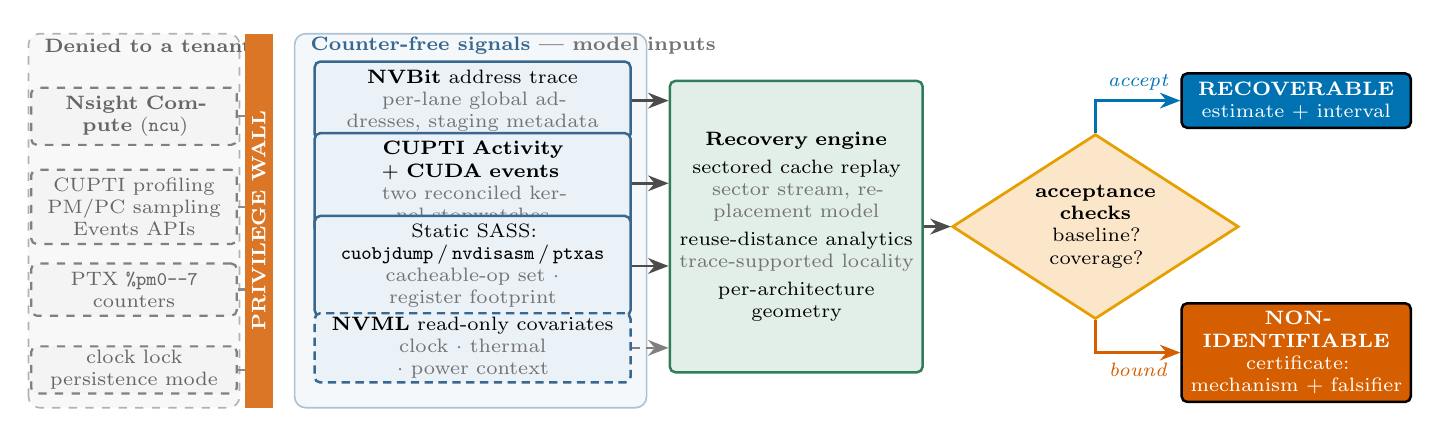
\begin{tikzpicture}
  \begin{scope}[on background layer]
    \fill[panel, fill=blockfill!60, draw=black!30, line width=0.6pt, dashed]
        (-8.80,0.20) rectangle (-6.12,4.95);
    \fill[panel, fill=panelblue, draw=surfaceedge!40, line width=0.6pt]
        (-5.42,0.20) rectangle (-0.95,4.95);
  \end{scope}
  \node[font=\scriptsize\bfseries, text=black!60, anchor=west] at (-8.72,4.80)
       {Denied to a tenant};
  \node[font=\scriptsize\bfseries, text=surfaceedge, anchor=west] at (-5.34,4.80)
       {Counter-free signals \nodedetail{--- model inputs}};

  \node (bd1) at (-7.46,3.90) [blocked, text width=24mm]
        {\textbf{Nsight Compute} (\texttt{ncu})};
  \node (bd2) at (-7.46,2.75) [blocked, text width=24mm]
        {CUPTI profiling\\PM/PC sampling\\Events APIs};
  \node (bd3) at (-7.46,1.70) [blocked, text width=24mm]
        {PTX \texttt{\%pm0--7}\\counters};
  \node (bd4) at (-7.46,0.68) [blocked, text width=24mm, inner ysep=1.4pt]
        {clock lock\\persistence mode};

  \fill[noid!85] (-6.05,0.20) rectangle (-5.70,4.95);
  \node[rotate=90, font=\scriptsize\bfseries, text=white] at (-5.875,2.58)
       {PRIVILEGE WALL};
  \foreach \n in {bd1,bd2,bd3,bd4} {
     \draw[denyline] (\n.east) -- (-6.05, 0 |- \n.east);
  }

  \node (s1) at (-3.16,4.10) [surf, text width=38mm]
        {\textbf{NVBit} address trace\\\nodedetail{per-lane global addresses, staging metadata}};
  \node (s2) at (-3.16,3.05) [surf, text width=38mm]
        {\textbf{CUPTI Activity} $+$ \textbf{CUDA events}\\\nodedetail{two reconciled kernel stopwatches}};
  \node (s3) at (-3.16,2.00) [surf, text width=38mm]
        {Static SASS: \texttt{cuobjdump}\,/\,\texttt{nvdisasm}\,/\,\texttt{ptxas}\\\nodedetail{cacheable-op set $\cdot$ register footprint}};
  \node (s4) at (-3.16,0.96) [surf, densely dashed, text width=38mm, inner ysep=1.4pt]
        {\textbf{NVML} read-only covariates\\\nodedetail{clock $\cdot$ thermal $\cdot$ power context}};

  \node (eng) at (0.95,2.50) [engine, text width=30mm, minimum height=37mm]
        {\textbf{Recovery engine}\\[2pt]
         sectored cache replay\\\nodedetail{sector stream, replacement model}\\[2pt]
         reuse-distance analytics\\\nodedetail{trace-supported locality}\\[2pt]
         per-architecture geometry};
  \draw[flow] (s1.east) -- (eng.west |- s1.east);
  \draw[flow] (s2.east) -- (eng.west |- s2.east);
  \draw[flow] (s3.east) -- (eng.west |- s3.east);
  \draw[flow, densely dashed, draw=black!50] (s4.east) -- (eng.west |- s4.east);

  \node (g) at (4.75,2.50) [gate, text width=18mm]
        {\textbf{acceptance checks}\\baseline?\\coverage?};
  \draw[flow] (eng.east) -- (g.west);

  \node (rec) at (7.30,4.10) [rectile, text width=27mm]
        {\textbf{RECOVERABLE}\\\textnormal{estimate $+$ interval}};
  \node (non) at (7.30,0.90) [nontile, text width=27mm]
        {\textbf{NON-IDENTIFIABLE}\\\textnormal{certificate:\\mechanism $+$ falsifier}};
  \draw[flow, draw=recblue] (g.north) |- (rec.west)
        node[pos=0.75, above, font=\scriptsize\itshape, text=recblue] {accept};
  \draw[flow, draw=noid] (g.south) |- (non.west)
        node[pos=0.75, below, font=\scriptsize\itshape, text=noid] {bound};
\end{tikzpicture}
\caption{\textbf{Counter-free observability under the privilege wall.}
Counter-bearing profiler surfaces and clock controls are unavailable when the
host keeps the post-CVE-2018-6260 default restriction in place. The pipeline
uses only permission-free signals from the tenant process, accepts recoverable
metrics only after predefined checks, and reports non-identifiable
metrics as mechanism-level certificates rather than unsupported point
predictions.}
\label{fig:overview}
\end{figure*}

This framing changes the role of a profiler substitute. Prior work offers
cycle-level simulation, analytic or learned performance prediction, roofline
analysis, and trace-driven cache modeling. Each is useful, but each gives up at
least one constraint in the tenant setting: privileged validation data,
configuration knowledge, clock control, or suite-average claims that do not say
which metrics are knowable for a particular run. We instead make the
non-privileged observation surface the premise.

\smallskip
\noindent\textbf{Contributions.}
\begin{enumerate}
\item We define a counter-free measurement method that uses only tenant-visible
signals and separates recoverable estimates from non-identifiable metrics by a
predefined set of checks.
\item We show that cache behavior has a structural boundary: reuse visible in
the global-address stream can be modeled by trace replay, while reuse staged
entirely on chip is erased from that stream.
\item We build a framework that applies the method at scale to a modern GPU
kernel benchmark, with per-kernel evidence availability, local reference
measurements used only for validation, and reproducible reporting.
\end{enumerate}

\section{Background and Related Work}
\label{sec:related}

\textbf{GPU execution and memory primer.} A GPU kernel executes as thousands
of threads grouped into 32-thread \emph{warps}; each thread occupies a
\emph{lane} of its warp and runs on one of the chip's \emph{streaming
multiprocessors} (SMs). Memory instructions target either \emph{global memory}
(device DRAM, addressable by all threads) or fast on-chip storage: registers
and the software-managed \emph{shared memory} (a scratchpad). Global accesses
pass through a two-level cache hierarchy (L1 per SM, L2 shared), and NVIDIA
caches move data in 32-byte \emph{sectors}, four per 128-byte cache line;
adjacent lane accesses are \emph{coalesced} into the minimal set of sector
requests. Profilers such as Nsight Compute report this machinery---hit rates,
sector traffic, \emph{occupancy} (the fraction of warp slots resident on each
SM), and instructions per cycle (IPC)---by reading hardware performance
counters, the privileged surface this paper does without.

\textbf{The measurement contract.} On a host that leaves
\texttt{NVreg\_Restrict\allowbreak Profiling\allowbreak To\allowbreak Admin\allowbreak Users}
enabled, an unprivileged process cannot use \textbf{Nsight Compute}, CUPTI
profiling interfaces, performance-monitor (PM) or program-counter (PC)
sampling, event and metric APIs, performance counters visible from PTX
(NVIDIA's virtual instruction set), or administrative clock
controls~\cite{nvidia_errnvgpuctrperm,nvidia_nsightcompute,nvidia_cupti}. The documented
remedies require root, a host-side driver option, or an administrative
container capability; all are outside the tenant's authority. The remaining
substrate is thinner but real: \textbf{NVBit} dynamic binary instrumentation,
which rewrites the tenant's own GPU binaries at load time to insert
measurement callbacks~\cite{villa2019nvbit,stephenson2015sassi}; unprivileged
\textbf{CUPTI Activity} records, timeline entries for kernel launches and
memory copies~\cite{nvidia_cupti_activity}; CUDA events, user-space GPU
stopwatches; \textbf{Nsight Systems} timelines~\cite{nvidia_nsightsystems};
static disassembly of SASS, the GPU's native machine
code~\cite{nvidia_cudabinutils}; correctness and memory tools such as
\textbf{compute-sanitizer}~\cite{nvidia_computesanitizer}; and read-only
\textbf{NVML} device-status covariates, the library behind
\texttt{nvidia-smi}~\cite{nvidia_nvml}.

\textbf{Simulator and model baselines.} GPGPU-Sim, Accel-Sim, NVArchSim, and
recent trace-driven core models reconstruct GPU behavior by modeling large
parts of the device~\cite{bakhoda2009gpgpusim,khairy2020accelsim,villa2021nvarchsim,huerta2025moderncores}.
Analytical and learned predictors, including the memory-/compute-warp-parallelism
(MWP/CWP) lineage, GPUMech, MDM, GCoM, and cross-architecture predictors,
produce fast estimates but are calibrated against privileged or
simulator-derived ground
truth~\cite{hong2009analytical,huang2014gpumech,wang2020mdm,lee2022gcom,ardalani2015xapp,lee2025neusight}.
Roofline analysis supplies a counter-light performance bound by capping a
kernel at peak compute and peak memory bandwidth, but hierarchical
GPU roofline variants still depend on per-level traffic
counts~\cite{williams2009roofline,yang2020hierarchical}. These systems answer
``what does a model predict?''; our question is ``what does the tenant's
observation surface determine?''

\textbf{Trace-driven cache modeling.} Reuse distance---the number of distinct
data blocks touched between two consecutive uses of the same block---gives a
classical bridge from address traces to cache behavior~\cite{mattson1970}. GPU
cache studies extend that idea to GPU hierarchies and memory
coalescing~\cite{nugteren2014gpucache,kiani2018reuse,arafa2020reuse,arafa2021pptgpu}.
Hierarchical reuse distance (HRD) preserves locality across sector and
coarser cache granularities~\cite{maeda2017hrd}. Separately, SHALOM studies
CPU multicore sharing locality; its taxonomy motivates our visible-stream
labels for local, sequential-sharing, concurrent-sharing, and private/cold
accesses~\cite{jiang2022shalom}.
The distinction here is not the use of a trace; it is that the trace is not
assumed complete. Modern tensor-core and attention-class kernels often stage
reuse through scratchpad, registers, or bulk-transfer machinery. When that reuse
does not re-enter the global-address stream, no HRD-style trace replay can
recover the missing hit behavior without an additional observation.

\textbf{Comparison metrics.} Table~\ref{tab:sotanorm} compares this paper's
reported metrics against the closest timing-backed GPU models. Metric-error
cells use GMRE, the geometric mean relative error over per-cell relative
errors, when paired predictions and references are available; otherwise, the
table keeps the baseline paper's reported unit and labels it in the cell. The
timing row reports elapsed or derived tool run time rather than accuracy.

\textbf{Instrumentation and microbenchmarking.} NVBit, SASSI, and programmable
assembly-level probes expose user-space instrumentation paths that do not
require counters~\cite{villa2019nvbit,stephenson2015sassi,huang2025neutrino}.
GPU microbenchmarking similarly uses self-timed experiments to infer hardware
geometry~\cite{wong2010demystifying,mei2017dissecting,jia2018volta,jarmusch2025blackwell}.
We use these facts as the observation and parameter substrate, then ask which
profiler metrics they identify for an actual kernel execution.

Table~\ref{tab:positioning} summarizes which baseline families provide the
tenant-visible evidence needed for run-specific measurement, uncertainty
intervals, per-family decisions, and explicit non-identifiability certificates.

\begin{table}[t]
\centering
\caption{\textbf{Baseline capabilities under the tenant-visible contract.}}
\label{tab:positioning}
\setlength{\tabcolsep}{1.4pt}
\renewcommand{\arraystretch}{1.1}
\scriptsize
\begin{tabular*}{\columnwidth}{@{\extracolsep{\fill}}>{\raggedright\arraybackslash}p{3.25cm}@{\hspace{4pt}}cccc@{}}
\toprule
& \textbf{\shortstack[c]{measures\\the run}}
& \textbf{\shortstack[c]{verified\\intervals}}
& \textbf{\shortstack[c]{per-family\\verdicts}}
& \textbf{\shortstack[c]{erasure\\certificates}}\\
\midrule
Cycle-level simulation~\cite{bakhoda2009gpgpusim,khairy2020accelsim} & \xm & \xm & \xm & \xm\\
Analytical/learned models~\cite{hong2009analytical,huang2014gpumech,wang2020mdm,lee2022gcom,lee2025neusight} & \xm & \xm & \xm & \xm\\
Roofline / speed-of-light~\cite{williams2009roofline} & \xm & \xm & \xm & \xm\\
Trace-driven cache models~\cite{nugteren2014gpucache,kiani2018reuse,maeda2017hrd,arafa2021pptgpu,arafa2020reuse} & \cm & \xm & \xm & \xm\\
Assembly-level probes~\cite{huang2025neutrino} & \cm & \xm & \xm & \xm\\
\textbf{This work} & \cm & \cm & \cm & \cm\\
\bottomrule
\end{tabular*}
\vspace{5pt}
\begin{minipage}{\columnwidth}
\fontsize{5.8}{6.5}\selectfont
\emph{Note.} A check indicates that the capability is available under the
tenant-visible observation surface without privileged counters. An erasure
certificate explicitly reports why a metric is not identifiable.
\end{minipage}
\end{table}

\section{Counter-Free Observation}
\label{sec:method}

The pipeline in Fig.~\ref{fig:overview} has three rules. First, deployed
features must come from surfaces available to an ordinary user. Second, every
estimate must pass predefined acceptance checks before it is reported. Third,
when the available signals do not identify a metric, the system reports the
missing mechanism rather than filling the gap with a fitted correction.

\subsection{Observation Surfaces}
\label{sec:signals}

The model inputs comprise four signal families. The address trace uses
\textbf{NVBit} to record global load and store addresses with active-lane
masks (which lanes of each warp participate in the access) and instruction
context. The timing path reconciles \textbf{CUPTI
Activity} records with CUDA events and discards measurements whose independent
stopwatches disagree. Static SASS inspection records cache-eligibility and
resource properties without executing the kernel. Read-only \textbf{NVML}
covariates record context such as clocks, temperature, and power, but the
deployed estimators do not treat those covariates as privileged counters.

The harness enforces the contract directly. Counter-derived features are
excluded, and clock-changing controls are disabled. The privileged profiler
appears only as an offline reference source on local hosts where the
experimenter controls the machine; it is never part of the tenant-visible
deployment path.

\subsection{Hierarchical Reuse-Distance Recovery}
\label{sec:cachemodel}

The richest counter-free signal is the memory-address stream. A cache access
hits when the data was used recently enough; base-layer reuse distance
formalizes this as the number of distinct sectors touched since the previous
access to the same sector~\cite{mattson1970}. The recovery engine uses a
sectorized HRD profile. Recorded lane addresses are first coalesced into
hardware-sector units following GPU cache-trace
practice~\cite{nugteren2014gpucache,kiani2018reuse}. The sector stream is then lifted
into coarser cache granularities and request-type channels following
HRD~\cite{maeda2017hrd}. A SHALOM-inspired locality tag records only the
local, sequential-sharing, concurrent-sharing, or private/cold reuse visible
in the global address stream before replay~\cite{jiang2022shalom}. The
cross-check compares the replayed cache state with an independent HRD profile.
The replay is intentionally narrow: it models
address-supported locality, not scheduling, timing, or hidden on-chip state.

\begin{figure*}[t]
\centering
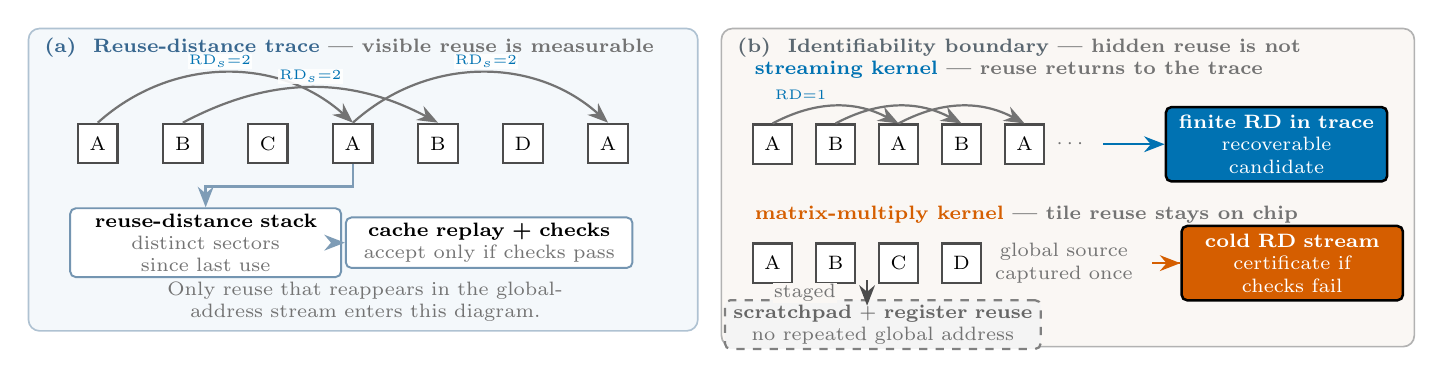
\begin{tikzpicture}[
  sect/.style={rectangle, draw=black!70, line width=0.8pt, fill=white,
               minimum size=5.0mm, inner sep=0.8pt, font=\scriptsize},
  arc/.style={->, black!55, line width=0.8pt},
  rd/.style={rectangle, draw=surfaceedge!70, fill=white, rounded corners=2pt,
             line width=0.7pt, align=center, font=\scriptsize, inner sep=2pt},
]
  \begin{scope}[on background layer]
    \fill[panel, fill=panelblue, draw=surfaceedge!40, line width=0.6pt]
        (-8.80,-1.82) rectangle (-0.30,2.02);
    \fill[panel, fill=panelwarm, draw=black!30, line width=0.6pt]
        (0.00,-2.02) rectangle (8.80,2.02);
  \end{scope}
  \node[font=\scriptsize\bfseries, text=surfaceedge, anchor=west] at (-8.72,1.78)
       {(a)~~Reuse-distance trace \nodedetail{--- visible reuse is measurable}};
  \node[font=\scriptsize\bfseries, text=panelgrey, anchor=west] at (0.08,1.78)
       {(b)~~Identifiability boundary \nodedetail{--- hidden reuse is not}};

  \node (p0) at (-7.92,0.56) [sect] {A};
  \node (p1) at (-6.84,0.56) [sect] {B};
  \node (p2) at (-5.76,0.56) [sect] {C};
  \node (p3) at (-4.68,0.56) [sect] {A};
  \node (p4) at (-3.60,0.56) [sect] {B};
  \node (p5) at (-2.52,0.56) [sect] {D};
  \node (p6) at (-1.44,0.56) [sect] {A};
  \draw[arc] (p0.north) to[bend left=42]
       node[pos=0.48, above=1.0pt, font=\tiny, text=recblue, fill=white,
            fill opacity=0.9, text opacity=1, inner sep=0.5pt] {$\mathrm{RD}_s{=}2$} (p3.north);
  \draw[arc] (p1.north) to[bend left=28]
       node[pos=0.50, above=1.0pt, font=\tiny, text=recblue, fill=white,
            fill opacity=0.9, text opacity=1, inner sep=0.5pt] {$\mathrm{RD}_s{=}2$} (p4.north);
  \draw[arc] (p3.north) to[bend left=42]
       node[pos=0.52, above=1.0pt, font=\tiny, text=recblue, fill=white,
            fill opacity=0.9, text opacity=1, inner sep=0.5pt] {$\mathrm{RD}_s{=}2$} (p6.north);
  \node (rdstack) at (-6.55,-0.70) [rd, text width=33mm]
       {\textbf{reuse-distance stack}\\\nodedetail{distinct sectors since last use}};
  \node (replay) at (-2.95,-0.70) [rd, text width=35mm]
       {\textbf{cache replay + checks}\\\nodedetail{accept only if checks pass}};
  \draw[flow, draw=surfaceedge!65] (p3.south) -- ++(0,-0.28) -| (rdstack.north);
  \draw[flow, draw=surfaceedge!65] (rdstack.east) -- (replay.west);
  \node at (-4.55,-1.45) [detail, align=center, text width=72mm]
       {Only reuse that reappears in the global-address stream enters this diagram.};

  \node[font=\scriptsize\bfseries, text=recblue, anchor=west] at (0.30,1.50)
       {streaming kernel \nodedetail{--- reuse returns to the trace}};
  \node (q0) at (0.65,0.55) [sect] {A};
  \node (q1) at (1.45,0.55) [sect] {B};
  \node (q2) at (2.25,0.55) [sect] {A};
  \node (q3) at (3.05,0.55) [sect] {B};
  \node (q4) at (3.85,0.55) [sect] {A};
  \node[font=\scriptsize, text=black!55] at (4.45,0.55) {$\cdots$};
  \draw[arc] (q0.north) to[bend left=28]
       node[pos=0.22, above=0.5pt, font=\tiny, text=recblue] {$\mathrm{RD}{=}1$} (q2.north);
  \draw[arc] (q1.north) to[bend left=28] (q3.north);
  \draw[arc] (q2.north) to[bend left=28] (q4.north);
  \node (vis) at (7.05,0.55) [rectile, text width=26mm]
       {\textbf{finite RD in trace}\\\textnormal{recoverable candidate}};
  \draw[flow, draw=recblue] (4.85,0.55) -- (vis.west);

  \node[font=\scriptsize\bfseries, text=noid, anchor=west] at (0.30,-0.35)
       {matrix-multiply kernel \nodedetail{--- tile reuse stays on chip}};
  \node (r0) at (0.65,-0.96) [sect] {A};
  \node (r1) at (1.45,-0.96) [sect] {B};
  \node (r2) at (2.25,-0.96) [sect] {C};
  \node (r3) at (3.05,-0.96) [sect] {D};
  \node (once) at (4.35,-0.96) [detail, align=center, text width=20mm]
       {global source\\captured once};
  \node (sm) at (2.05,-1.74) [blocked, text width=38mm, inner ysep=1.7pt]
       {\textbf{scratchpad $+$ register reuse}\\
        \nodedetail{no repeated global address}};
  \draw[flow] (1.85,-1.18) -- (1.85,-1.50);
  \node[font=\scriptsize, text=black!55, fill=panelwarm, inner sep=0.6pt, anchor=east]
       at (1.48,-1.34)
       {staged};
  \node (era) at (7.25,-0.96) [nontile, text width=26mm]
       {\textbf{cold RD stream}\\\textnormal{certificate if checks fail}};
  \draw[flow, draw=noid] (once.east) -- ++(0.35,0) |- (era.west);
\end{tikzpicture}
\caption{\textbf{Why a reuse-distance trace succeeds and fails.} Visible reuse
creates finite reuse distances that can be replayed. Reuse staged in scratchpad
or registers can change hardware hit behavior without producing additional
global-address observations, creating a structural erasure mechanism.}
\label{fig:reuse}
\end{figure*}

\subsection{Acceptance Checks and Certificates}
\label{sec:gates}

A bare estimate is not enough. Each recoverable metric is compared with the
strongest available baseline and, when calibrated intervals are meaningful, its
coverage is checked on held-out evidence using conformal prediction, a
distribution-free technique that calibrates interval widths so that a stated
fraction of held-out truths falls inside them~\cite{vovk2005alrw}. A failed
baseline, coverage, or robustness check produces an explicitly unsupported
estimate, not a softened pass.

For a non-identifiable quantity, the output is a certificate. The certificate
contains the affected metric, the hiding mechanism, the bounded evidence in
hand, and the non-privileged observation that would falsify the verdict. This
borrows the language of structural identifiability~\cite{villaverde2016structural}
but applies it to performance observability: before estimating a metric, the
system asks whether the available signals determine it at all.

\section{Identifiability Map}
\label{sec:map}

The map applies these checks to the profiler quantities that performance analysts
normally consult: traffic between cache levels, cache hit rates, memory-system
traffic, bandwidth, cycles, occupancy, instruction throughput, and related
derived quantities. The result is a boundary: metrics tied directly to the
recorded global-address stream can enter the recoverable tier. Metrics governed
by hidden controller behavior, scheduler state, dynamic frequency, or on-chip
staging receive certificates.

Throughout the map, a metric receives one of three verdicts:
\emph{recoverable} (the estimate passes every predefined check),
\emph{outside support} (an estimator exists but fails an accuracy, coverage,
or robustness check), or \emph{non-identifiable} (the required information is
structurally absent from the observation surface, so the metric receives a
certificate). A \emph{cell} denotes one kernel--input-shape configuration.

\medskip
\noindent\begin{minipage}{\columnwidth}
\centering
\textbf{\footnotesize Essential NCU-Metric Observability Map}\\[-1pt]
\setlength{\tabcolsep}{2pt}
\renewcommand{\arraystretch}{1.04}
\fontsize{5.9}{6.55}\selectfont
\begin{tabular*}{\columnwidth}{@{\extracolsep{\fill}}>{\raggedright\arraybackslash}p{2.15cm}>{\raggedright\arraybackslash}p{5.35cm}@{}}
\toprule
\textbf{Metric family} & \textbf{Result under tenant-visible signals} \\
\midrule
L1$\rightarrow$L2 read sectors &
RTX 5060 recoverable, GMRE $2.7{\times}10^{-12}$ over 39 held-out cells;
RTX 3090 Ti remains outside support because p90 error reaches $0.51$.\\
L1$\rightarrow$L2 write sectors &
Recoverable on both GPUs; RTX 5060 GMRE $5.1{\times}10^{-7}$ with 90/95\%
coverage 35/39 and 36/39; RTX 3090 Ti has 19/20 exact cells.\\
L1 sector hit rate &
Outside support: Blackwell intervals reach the width floor, and Ampere has
GMRE $0.89$ over 30 cells.\\
L2 sector hit rate &
Family-dependent: streaming kernels have median error $0.04$; staged-reuse
families range from $0.13$ to $0.92$ because reuse stays on chip.\\
DRAM traffic and bandwidth &
Not identifiable without a non-counter view of controller transactions,
coalescing/compression outcomes, and clock-stable byte timing.\\
Cycles, IPC, occupancy, throughput &
Not identifiable from address traces because the missing state is scheduler
residency, dynamic frequency, or hidden memory-system traffic.\\
\bottomrule
\end{tabular*}
\vspace{3pt}
\begin{minipage}{\columnwidth}
\raggedright
\fontsize{5.6}{6.2}\selectfont
\emph{Note.} GMRE is geometric mean relative error; p90 is the 90th-percentile
relative error. An interval at the \emph{width floor} is maximally wide and
therefore uninformative. This compact map summarizes the eleven-metric result
set while keeping the detailed state-of-the-art comparison in
Table~\ref{tab:sotanorm}.
\end{minipage}
\end{minipage}
\medskip

The recoverable tier is intentionally narrow. The read-sector path is exact on
Blackwell, the write-sector path clears the checks on both GPU generations, and
the L1 hit-rate estimator remains outside support when its uncertainty or its
handling of bypass-class loads (loads that skip L1 entirely) exceeds the
stated budget. This ordering matters: the
same address trace can determine traffic counts while still lacking enough
information to determine every hit rate.

\begin{table}[t]
\centering
\caption{\textbf{L2 hit-rate recoverability by kernel family.}}
\label{tab:l2family}
\setlength{\tabcolsep}{3pt}
\renewcommand{\arraystretch}{1.15}
\scriptsize
\begin{tabular*}{\columnwidth}{@{\extracolsep{\fill}}l@{\hspace{4pt}}ccc>{\raggedright\arraybackslash}p{2.65cm}@{}}
\toprule
\textbf{Kernel family} & $n$ & \textbf{median error} &
$\times$\textbf{threshold} & \textbf{Verdict: hidden mechanism} \\
\midrule
memory streaming & 6 & $0.04$ & $0.8\times$ &
\textcolor{recblue}{\textbf{recoverable}}: reuse re-traverses global memory \\
\addlinespace[1.5pt]
reduction / normalize & 7 & $0.32$ & $5.9\times$ &
\textcolor{noid}{\textbf{not identifiable}}: cross-group partial-sum reuse unseen \\
\addlinespace[1.5pt]
intermediate buffers & 7 & $0.13$ & $2.4\times$ &
\textcolor{noid}{\textbf{not identifiable}}: cache-resident staging buffers unseen \\
\addlinespace[1.5pt]
matrix multiply & 9 & $0.92$ & $16.7\times$ &
\textcolor{noid}{\textbf{not identifiable}}: operand tiles staged on chip \\
\addlinespace[1.5pt]
register spill & 0 & --- & --- &
\textcolor{noid}{\textbf{not identifiable}}: no observed case to score; reuse is thread-private \\
\bottomrule
\end{tabular*}
\vspace{5pt}
\begin{minipage}{\columnwidth}
\fontsize{5.8}{6.5}\selectfont
\emph{Note.} Errors are absolute hit-ratio fractions for the RTX 5060 L2 family
study. The fixed acceptance threshold is $0.055$. An independent checker agrees
on all 29 scoreable cells; the suite spans 70 admitted kernel/shape cells across
the two GPUs, and the RTX 3090 Ti confirms the same streaming-versus-staged
boundary structurally.
\end{minipage}
\end{table}

Table~\ref{tab:l2family} applies this boundary to the L2 hit ratio. Streaming
kernels expose repeated sectors directly in the address stream and remain below
the threshold. The families that dominate modern AI kernels do not: reductions
and normalization reuse partial sums across cooperating groups, intermediate
buffers can remain cache-resident between visible accesses, matrix multiply
stages operand tiles through shared memory and registers after one global fetch,
and register-spill reuse is thread-private. An HRD replay sees the global source
traffic but not the staged reuse. A fitted correction can match a cohort only by
importing assumptions not present in the observation surface; the map therefore
treats such outcomes as certificates unless the additional staging observation
is present and passes the same checks. For matrix multiply, for example, the
visible trace records the global fetch of operand tiles, but the subsequent
scratchpad destinations, register reuse, and on-chip residency do not generate
new global-address observations. The staging metadata available in the current
tenant trace identifies instruction context and global-source behavior; it does
not yet expose enough destination or residency information to identify the L2
hits created by that staged reuse.

\subsection{Validation Discipline}
\label{sec:microbench}

The validation suite is organized by metric family and by GPU generation. The
two test devices are an RTX 5060, from NVIDIA's recent Blackwell generation
(compute capability sm\_120), and an RTX 3090 Ti, from the older Ampere
generation (sm\_86). The suite comprises five L2 kernel families, 70 admitted
kernel/shape cells across the two GPUs, and separate held-out cohorts for
traffic recovery. Each cell is scored against a local
Nsight Compute reference measurement. For each metric, validation compares the
counter-free estimate with the local privileged reference measurement and
records whether the predefined checks pass. The reported metrics follow the
conventions used by the
simulation and analytical-modeling literature, but the decision rule is per
metric and per family rather than a suite average. Correlation is treated as
descriptive only: large dynamic ranges can make a failed estimator look
aligned, so acceptance depends on metric-specific error, coverage, and
robustness criteria.

The kernels are deliberately split into two groups. Synthetic microbenchmarks
isolate one mechanism at a time: sector coalescing, read/write traffic, cache
eligibility, hierarchical reuse distance, staged on-chip reuse, and stopwatch
agreement.
Native benchmark kernels then test whether the same evidence path survives
real operator structure: tensor-core tiles, attention-style reuse,
normalization and reduction, quantization, and fused movement. This separation
keeps the validation falsifiable. A microbenchmark can diagnose which
mechanism failed, while a native kernel tests whether that mechanism remains
visible once scheduling, fusion, and library code are present.

The retained microbenchmark results show both sides of the decision rule. On
the RTX 5060, L1$\rightarrow$L2 read sectors are recovered exactly over 39
held-out kernel configurations, with GMRE $2.7{\times}10^{-12}$ and no fitted
parameters. L1$\rightarrow$L2 write sectors are also accepted, with Blackwell
GMRE $5.1{\times}10^{-7}$ and verified 90/95\% coverage of 35/39 and 36/39.
On the RTX 3090 Ti, writes remain accepted: p90 error $0.00$, 19/20 exact
cells, mean absolute percentage error (MAPE) of 5\%, and Pearson correlation
$r{>}0.999$. The same cross-architecture pass does not
hold for every metric. Ampere read sectors still show 11/13 exact cells,
MAPE 19\%, and $r{=}0.94$, but remain outside support because two Ampere L2
mechanisms---the persisting-window carveout, a region of L2 reserved for
designated data, and full-line fetch granularity, which fetches the whole
128-byte line rather than individual sectors---push p90 error to $0.51$
against the $0.25$ target. L1 hit rate is outside the supported region on
both GPUs: the Blackwell interval reaches
the width floor, and the Ampere closure has GMRE $0.89$ over 30 cells. L2 hit
ratio exposes the staged-reuse boundary directly: Blackwell has family median
errors from $0.04$ to $0.92$ and only $r{=}0.38$ over 29 cells, while the Ampere
fit reaches aggregate GMRE $0.064$ but remains a fitted aggregate because leave-one-out and
leave-one-kernel-out checks move it by $0.34$ and $0.71$. The Ampere result is
therefore used as a structural confirmation of the hidden-reuse boundary, not
as a promoted fitted measurement: the mechanism matches across generations, but
the fitted number is too sensitive to the held-out kernel.

\begin{figure*}[t]
\centering
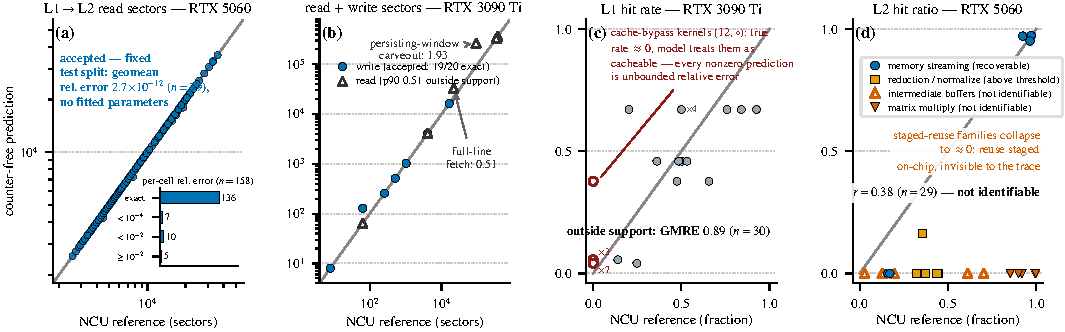
\includegraphics[width=\textwidth]{figures/fig_microbench.pdf}
\vspace{-3pt}
\caption{\textbf{Microbenchmark validation against local Nsight Compute
references.} Panels show Blackwell read-sector recovery, Ampere read/write
traffic, Ampere L1 hit-rate boundary, and Blackwell L2 hit ratio by family.
Accepted estimates follow the diagonal; unsupported estimates and certified
families show the per-cell failure modes that suite averages would hide.}
\label{fig:microbench}
\end{figure*}

\section{Framework at Benchmark Scale}
\label{sec:framework}

The framework packages the method for an industrial GPU-kernel benchmark
environment. The benchmark side supplies native CUDA/CUTLASS profiling targets
for the workloads under study, numerical-correctness checks, and per-kernel
metadata. The measurement side applies the permission-free signals from
Section~\ref{sec:signals} to each kernel and records why evidence is absent:
host unavailable, kernel failure, unsupported signal, or missing reference
measurement. Missing data are therefore named explicitly rather than silently
omitted.

The benchmark target is SOL-ExecBench, a speed-of-light suite that scores
real-world GPU kernels against hardware limits~\cite{nvidia2026solexecbench}.
Its 235 problems span four genres: two difficulty tiers that the suite names
L1 (94 problems) and L2 (82)---a labeling unrelated to the L1/L2 caches---plus
quantization (Quant, 33) and FlashInfer-derived (FIB, 26) kernels.
The upstream references are not ideal profiling targets
because Python dispatch, JIT compilation, and framework scheduling can share a
timeline with the kernel. We therefore use native CUDA/CUTLASS ports for
profiling, so both the counter-free surfaces and the local reference measurement
attach to the same executable kernel body.

\textbf{Local reference measurements.} Nsight Compute is restricted to local
machines where the experimenter controls the host. It supplies labels for
validation and calibration only; it is not invoked on the target tenant path.
This separation is essential: the deployed framework must run under the same
non-privileged contract that motivates the paper.

\textbf{Reporting rules.} Tables and figures use fixed metric names, units,
baselines, and acceptance rules. A metric is reported or marked outside support
only under those stated rules. Table~\ref{tab:sotanorm} follows the same
convention with GMRE used for metric-error cells.

The evaluated native benchmark set includes 127 correctness-passing Blackwell
ports and 178 completed Ampere kernel instances. Evidence availability---the
number of SOL-ExecBench kernels for which the counter-free pipeline produced
usable signals---reaches 222 kernels on the RTX 5060 and 225 on the RTX 3090 Ti. The cache-prediction
cohorts require both counter-free traces and repeatable local NCU reference
measurements. On that subset, calibrated hit-rate prediction remains within the
cohort thresholds: on the RTX 3090 Ti main set ($n{=}34$), leave-one-out mean
absolute error is $0.033 \le 0.05$ for L1 and $0.055 \le 0.06$ for L2; on the
RTX 5060 held-out cohort, the corresponding errors are $0.036$ and $0.038$.
The stress cases ($n{=}1$ and $n{=}2$) remain within their looser threshold.
These are benchmark-scale calibrated-prediction results, not per-kernel
recovery verdicts: the L2 cohort is threshold-sensitive, and staged-reuse
kernels still receive the family-level interpretation from Table~\ref{tab:l2family}.

\begin{figure*}[t]
\centering
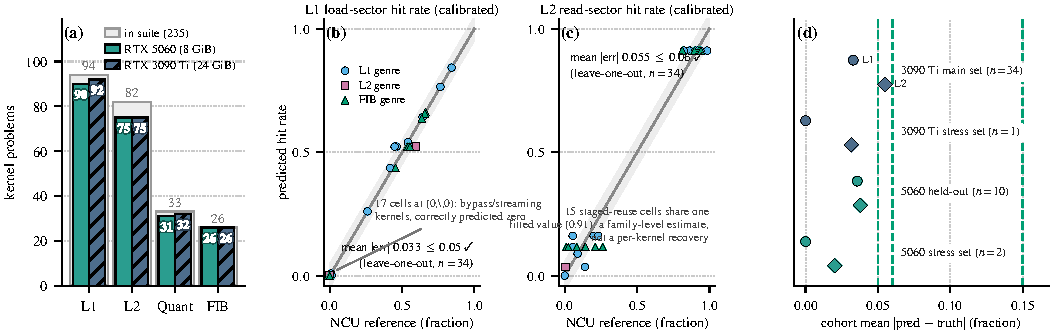
\includegraphics[width=\textwidth]{figures/fig_framework.pdf}
\vspace{-3pt}
\caption{\textbf{Benchmark-scale framework evidence.} Panel (a) reports
SOL-ExecBench availability by genre on both GPUs.
Panels (b)--(c) compare calibrated L1 and L2 hit-rate predictions with local
Nsight Compute references on the RTX 3090 Ti cohort. Panel (d) summarizes
cohort mean absolute errors against the thresholds shown in the panel; L1
points are circles and L2 points are diamonds.}
\label{fig:framework}
\end{figure*}

\section{Evaluation Protocol}
\label{sec:evaluation}

This section consolidates the protocol behind the results of
Sections~\ref{sec:map} and~\ref{sec:framework} and places them beside the
closest prior models. Table~\ref{tab:evaluation} lists the evaluation
questions and the evidence
reported for each one. Each question has a fixed measurement, acceptance check,
and failure reason. This prevents post-hoc reshaping of claims: a metric either
passes the stated checks, remains outside support with the failed criterion named, or
receives a non-identifiability certificate.

\begin{table}[!h]
\centering
\caption{\textbf{Evaluation questions and reported evidence.}}
\label{tab:evaluation}
\setlength{\tabcolsep}{3pt}
\renewcommand{\arraystretch}{1.12}
\scriptsize
\begin{tabular*}{\columnwidth}{@{\extracolsep{\fill}}>{\raggedright\arraybackslash}p{2.1cm}>{\raggedright\arraybackslash}p{5.5cm}@{}}
\toprule
\textbf{Question} & \textbf{Reported evidence} \\
\midrule
Interconnect traffic & read/write-sector error, interval coverage, and support decision \\
L1 behavior & hit-rate error, interval width, and cache-eligibility check \\
L2 behavior & per-family error, support decision, and certificate when staged reuse is not visible \\
Benchmark scale & per-architecture coverage, named exclusions, and cohort-level decisions \\
Tenant portability & which permission-free signals are available when privileged profilers are excluded \\
\bottomrule
\end{tabular*}
\vspace{5pt}
\begin{minipage}{\columnwidth}
\fontsize{5.8}{6.5}\selectfont
\emph{Note.} Each row states the evidence used to report an estimate, mark it
outside support, or support a non-identifiability certificate.
\end{minipage}
\end{table}

\begin{table}[!h]
\centering
\caption{\textbf{Metric-level comparison against timing-backed GPU models.}}
\label{tab:sotanorm}
\setlength{\tabcolsep}{1.8pt}
\renewcommand{\arraystretch}{1.10}
\fontsize{6.05}{6.9}\selectfont
\begin{tabular*}{\columnwidth}{@{\extracolsep{\fill}}>{\raggedright\arraybackslash}p{2.55cm}*{3}{>{\centering\arraybackslash}p{1.72cm}}@{}}
\toprule
\textbf{NCU metric(s)} &
\textbf{\shortstack{This work\\error/runtime}} &
\textbf{\shortstack{Nugteren\\'14\\error/runtime}} &
\textbf{\shortstack{Accel\\Sim'20\\error/runtime}} \\
\midrule
\sotametric{L1 sector hit rate}{l1tex__t_sector_hit_rate.pct} &
\shortstack{0.89\\{\tiny outside support}} &
\shortstack{6.4/8.3 pp} &
\shortstack{0.76\\NRMSE}
 \\
\addlinespace[2pt]
\sotametric{L1 to L2 read sectors}{l1tex__m_xbar2l1tex_read_sectors_mem_lg_op_ld.sum} &
\shortstack{$2.7{\times}10^{-12}$} &
 &
\shortstack{0.03\\NRMSE}
 \\
\addlinespace[2pt]
\sotametric{L1 to L2 write sectors}{l1tex__m_l1tex2xbar_write_sectors_mem_lg_op_st.sum} &
\shortstack{$5.1{\times}10^{-7}$} &
 &
 \\
\addlinespace[2pt]
\sotametric{L2 sector hit rate (calibrated cohorts)}{lts__t_sector_hit_rate.pct} &
\shortstack{\textbf{0.063}\\\textbf{0.069}\\{\tiny cohort}} &
\shortstack{0.117\\0.414\\GMRE} &
\shortstack{0.47\\NRMSE}
 \\
\addlinespace[2pt]
Tool runtime \newline
\hbox{\tiny\color{black!55}(elapsed time or derived run time)} &
\shortstack{60 s/kernel} &
\shortstack{cutcp: 10 s model\\+ 240 s Ocelot trace} &
\shortstack{80 s/1M warp instr.\\48 h trace gen.} \\
\bottomrule
\end{tabular*}
\vspace{5pt}
\begin{minipage}{\columnwidth}
\fontsize{5.8}{6.5}\selectfont
\emph{Note.} Metric rows report error against hardware or simulator ground
truth for NCU metrics under the stated support or cohort scope; the final row
reports exact elapsed or derived tool timings. GMRE is geometric mean relative error,
computed over per-cell relative errors. When a baseline cannot be converted to
GMRE from source-reported pairs, the table keeps the paper's original unit:
pp denotes percentage-point hit-rate error and NRMSE denotes normalized root
mean squared error. Blank cells indicate that the source does not report a
timing-backed comparable metric. The Nugteren L1 pp values correspond to the
16KB and 48KB cache configurations reported in the source. The L2 row uses the
calibrated-cache comparison cohorts shared with the HPCA'14 reuse-distance
baseline; paired L2 values are for the Ampere (sm\_86) then the Blackwell
(sm\_120) GPU, while
Table~\ref{tab:l2family} gives the family-level support boundary. Bold marks
the lowest GMRE where units are directly comparable.
Sources:
Nugteren et al.~\cite{nugteren2014gpucache} and
Accel-Sim~\cite{khairy2020accelsim}.
\end{minipage}
\end{table}
\FloatBarrier

The tables separate measured quantities from interpretation criteria. A metric
is reported as recoverable only when it satisfies the stated error, coverage,
and robustness checks. Otherwise, the evaluation names the reason the metric
cannot be identified from tenant-visible signals.

\section{Discussion and Limitations}
\label{sec:discussion}

\textbf{What the boundary means.} The limit on counter-free observability is
structural, not merely statistical. A failed cache estimate may indicate a
modeling defect, but it may also indicate that the relevant information never
entered the observation surface. The certificate form forces that distinction.
It tells the practitioner whether a metric can be reported now, and it tells
tool builders which additional non-privileged observation would make the metric
testable.

\textbf{Why bounded reporting matters.} A profiler substitute that always returns a
number is attractive but dangerous. It hides the difference between a
recoverable counter, a calibrated cohort prior, and a structurally erased
quantity. This work treats support boundaries as part of the measurement result.
Marking an unsupported estimate preserves the validity of accepted claims and prevents
suite-average accuracy from masking per-family failure.

\textbf{Evidence discipline.} Accuracy targets and workload partitions are fixed
before scoring. Intervals are checked for coverage, recovered counts are
cross-checked by independent calculations, and fitted corrections stay outside
support when they fail holdout robustness. Several quantities therefore remain
reported as unsupported even when a point estimate is numerically close; the
paper treats those misses as results, not as text to be optimized away.
The exact timings in Table~\ref{tab:sotanorm} are tool runtimes; architectural
cycles, IPC, and throughput remain outside support when tenant-visible timers
agree but the non-idle SM clock can still span 1688--2762 MHz.

\textbf{External validity.} The privileged reference requires local machines
where the experimenter controls profiler permissions. A rented datacenter
container can run the counter-free surfaces, but it cannot produce a privileged
reference under the same tenant contract. Datacenter deployment is therefore an
availability and portability exercise; counter-level validation on those hosts
requires administrator cooperation and is outside the tenant-only threat model.

\section{Conclusion}

This paper reframes GPU profiling under counter lockdown as an identifiability
problem. Given only legal tenant-visible signals, some quantities can be
recovered with predefined checks and uncertainty evidence; others are erased by
hardware behavior that never reaches the global-address trace. The resulting
profiler is not merely a counter surrogate. It is a boundary-drawing system:
recover what the observation surface determines, mark what it does not, and
name the extra observation required to change the verdict. The results show
machine-precision L1$\rightarrow$L2 read-sector recovery on Blackwell,
coverage-checked write-sector recovery on both GPUs, streaming-kernel L2
hit-ratio recovery within threshold, and benchmark-scale availability of
222 and 225 SOL-ExecBench kernels on the two evaluated GPUs.

\providecommand{\BIBdecl}{}
\renewcommand{\BIBdecl}{\fontsize{7.75}{8.35}\selectfont}
\bibliographystyle{IEEEtran}
\bibliography{refs}

\end{document}
